\documentclass[../AnalysisNoteJBuxton.tex]{subfiles}
\begin{document}

\subsection{Cascade Reconstruction}
\label{CascadeReconstruction}

The reconstruction of $\Xi$ particles is one step above V0 reconstruction.  V0 particles are topologically reconstructed by searching for the charged daughters' tracks into which they decay.  With $\Xi$ particles, we search for the V0 particle and charged daughter into which the $\Xi$ decays.  In the case of $\Xi^{-}$, we search for the $\Lambda$ (V0) and $\pi^{-}$ (track) daughters.  We will refer to this $\pi$ as the ``bachelor $\pi$".  The reconstruction of $\Xi$, and the specific cuts used will be included in future versions of this note.

\begin{figure}[h]
  \centering
  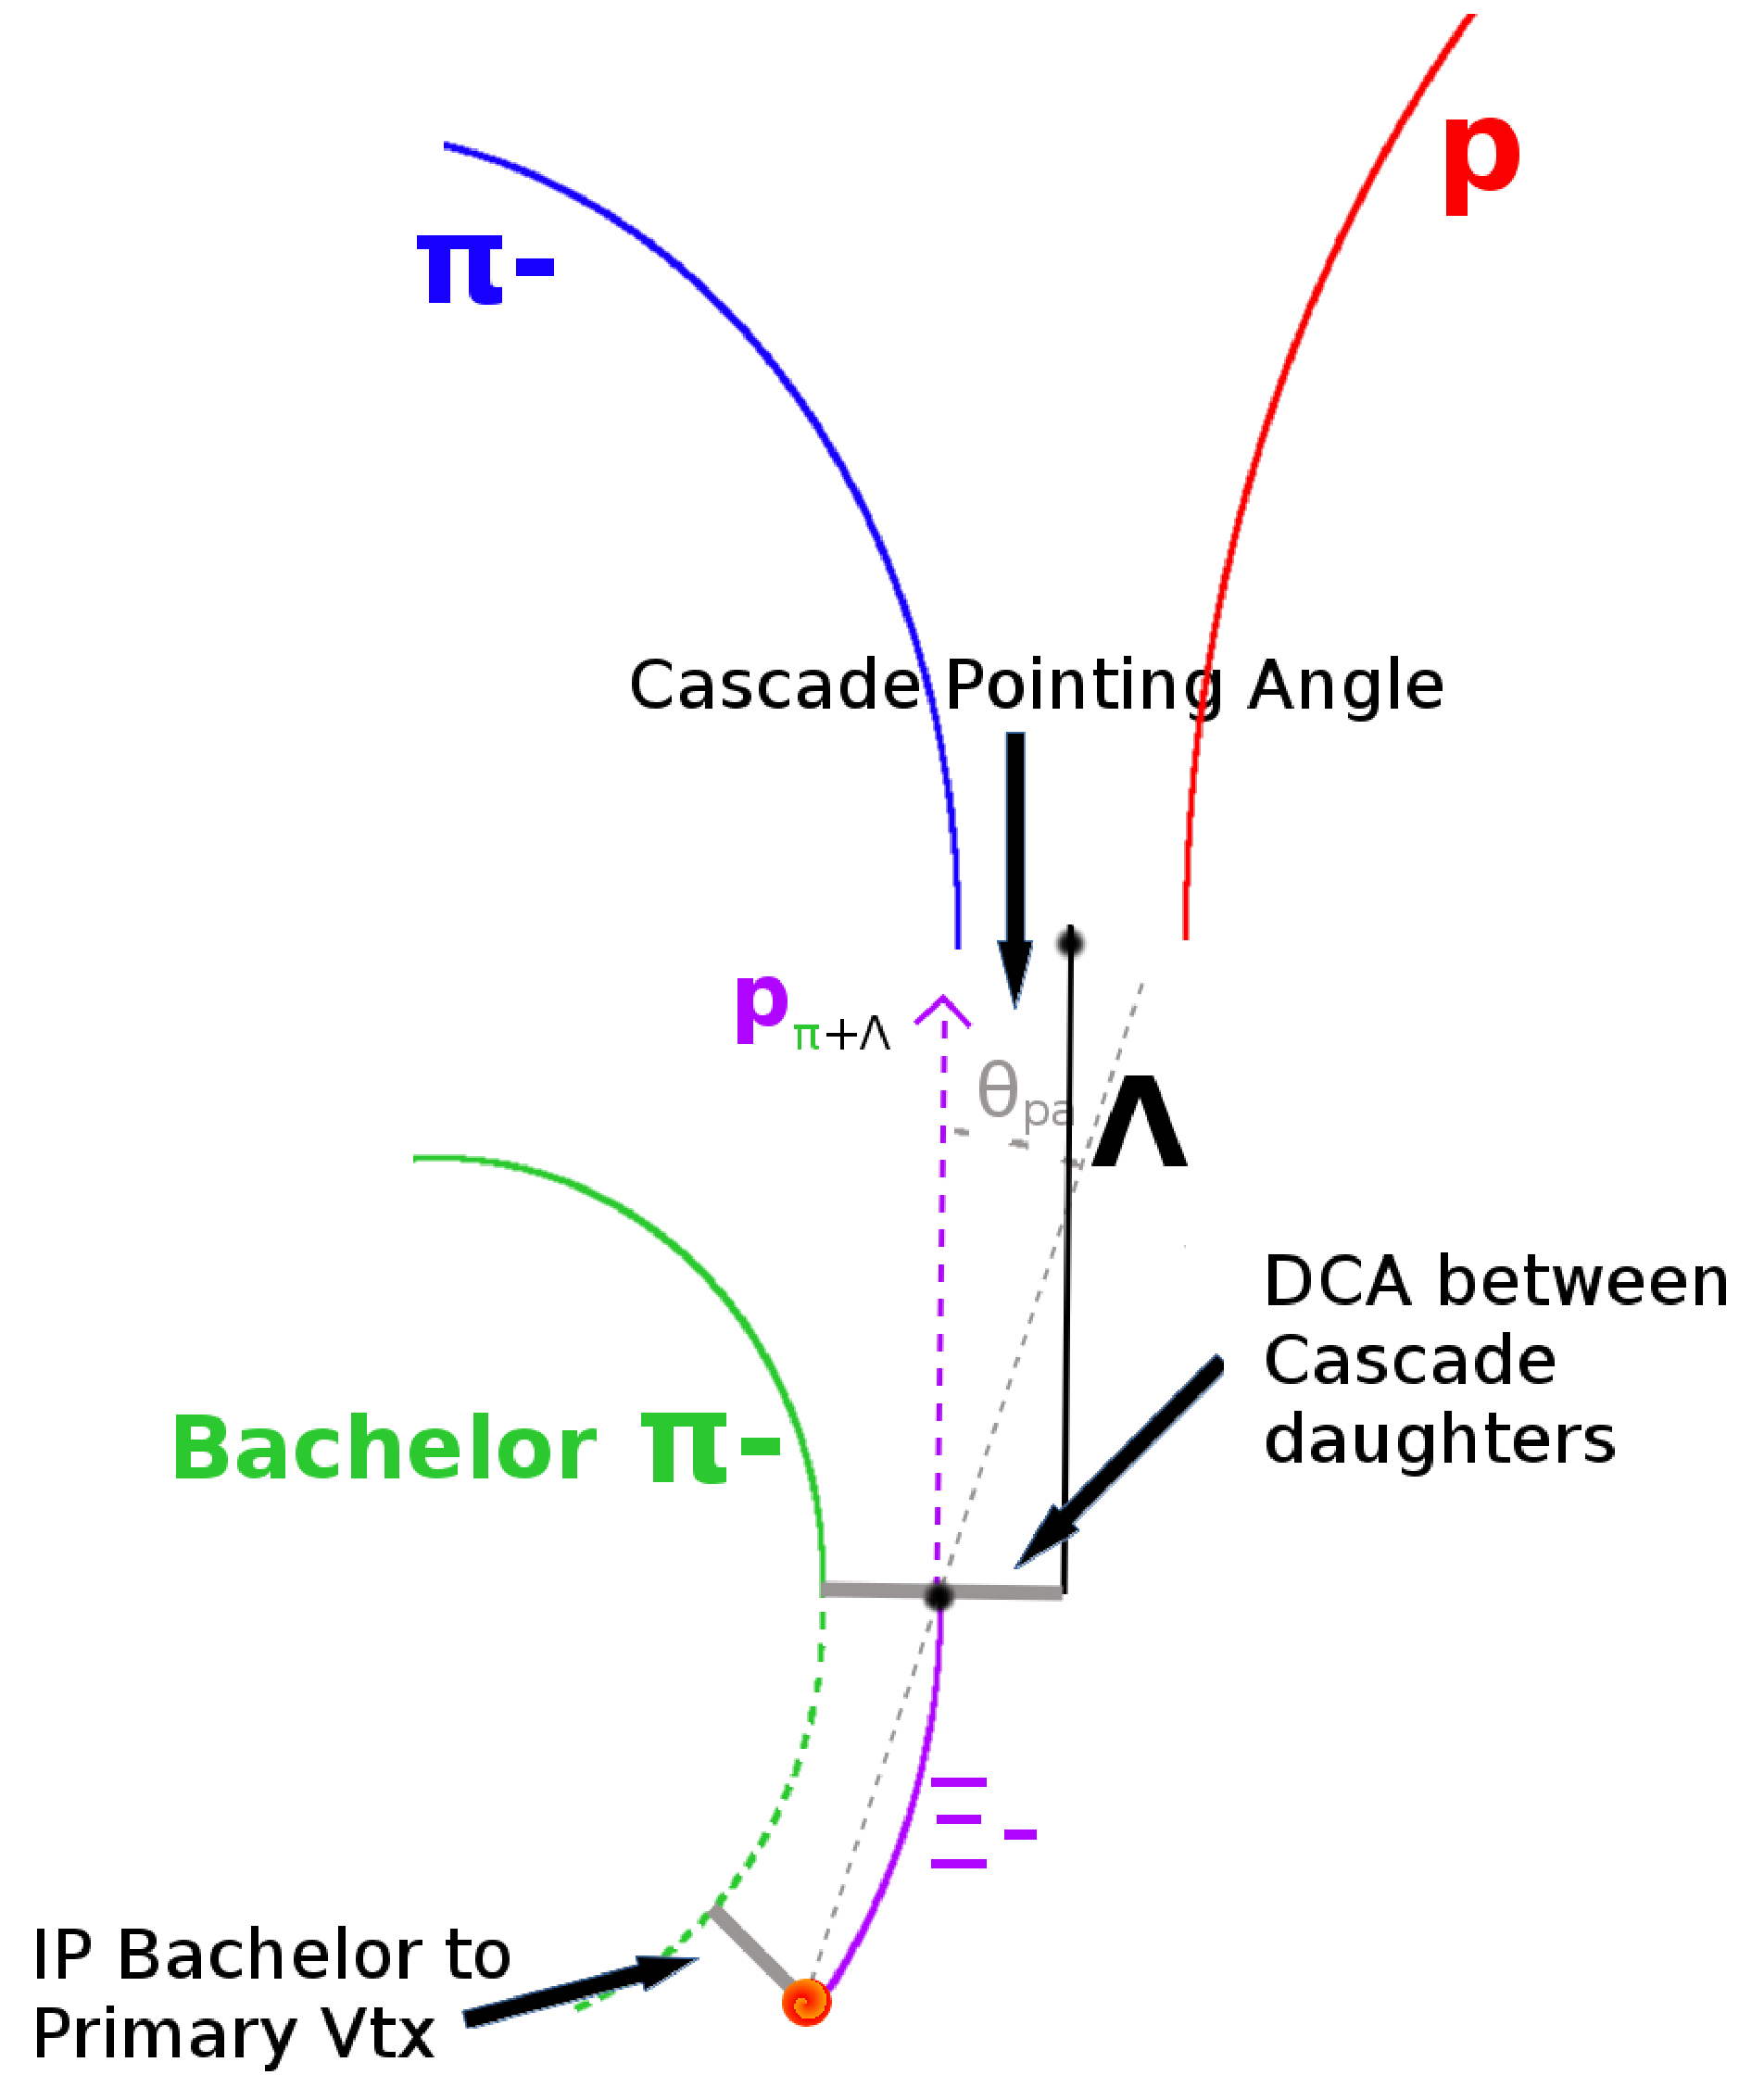
\includegraphics[width=0.5\textwidth]{3_DataSelection/Figures/XiCuts.pdf}
  \caption[$\Xi$ Reconstruction]{$\Xi$ Reconstruction}
  \label{fig:XiReconstruction}
\end{figure}

\end{document}